\section{Experiments}


We evaluate our algorithm on a range of continuous control tasks from OpenAI Gym \cite{gymopenai} and the meta world benchmark \cite{yu2020meta} that both use  the physics engine MuJoCo \cite{mujoco} (version 1.5). 
First, we benchmark ACC against strong methods that do not use environment specific hyerparameters.
Then we compare the performance of TQC with a fixed number of dropped targets per network with that of ACC.
Next, we evaluate the effect of more critic updates for ACC and show results in the sample efficient regime.
Further, we study the effect of ACC on the accuracy of the value estimate, and investigate the generality of ACC by applying it to TD3.







We implemented ACC on top of the PyTorch code published by the authors\footnote{\url{https://github.com/bayesgroup/tqc_pytorch}} to ensure a fair comparison.
While in general a safe strategy is to use a very high value for $d_{max}$ as it gives ACC more flexibility in choosing the right amount of bias correction we set it to $d_{max}=5$, which is the maximum value used by TQC for the number of dropped targets in the original publication.
At the beginning of the training we initialize $\beta = 2.5$ and set the step size parameter to $\alpha=0.1$.
After $T_\beta = 1000$ steps since the last update and when the next episode finishes, $\beta$ is updated with a batch that stores the most recent state-action pairs encountered in the environment and their corresponding observed discounted returns. 
After every update of $\beta$ the oldest episodes in this stored batch are removed until there are no more than $5000$ state-action pairs left.
This means that on average $\beta$ is updated with a batch whose size is a bit over $5000$. 
The updates of $\beta$ are started after $25000$ environment steps and
the moving average parameter in the normalization of the $\beta-$update is set to $0.05$. 
The  first $5000$ environment interactions are generated with a random policy after which learning starts.
We did not tune most of these additional hyperparameters and some choices are directly motivated by the environment (e.g. setting $T_\beta$ to the maximum episode length). Only for $\alpha$ we tested a few different choices but found that for reasonable values it does not have a noticeable influence on performance. 
% We spend only a very limited amount of computation time into the tuning of the previously mentioned hyperparameters.
All hyperparameters of the underlying TQC algorithm  with $N=5$ critic networks were left unchanged.




Compared to TQC the additional computational overhead caused by ACC is minimal because there is only one update to $\beta$ that is very cheap compared to one training step of the actor-critic and there are at least $T_\beta =1000$ training steps in between one update to $\beta$.





During training, the policy is evaluated every 1,000 environment steps by averaging the episode returns of $10$ rollouts with the current policy. For each task and algorithm we run 10 trials each with a different random seed.



\subsection{Comparative Evaluation}




We compare ACC to the state of the art continuous control methods SAC \cite{SAC} (with learned temperature parameter \cite{SACalgapp}) and TD3 \cite{td3} on six OpenAI Gym continuous control environments.
To make the different environments comparable we normalize the scores by dividing the achieved return by the best achieved return among all evaluations points of all algorithms for that environment.

Figure \ref{fig:comparative_aggregated_results}a)  shows the aggregated data efficiency curve over all $6$ tasks computed with the method of \cite{agarwal2021deep}, where the interquantile mean (IQM) ignores the bottom and top $25$\% of the runs across all games and computes the mean over the remaining. 
The absolute performance of ACC for each single task can be seen in Figure \ref{fig:ablation_const_number_dropped_atoms_single_curves}.
Overall, ACC reaches a much higer performance than SAC and TD3.


\subsection{Robotics Benchmark}
To investigate, if ACCs strong performance also translates into robotics environments, we evaluate ACC and SAC on $12$ of the more challenging tasks in the Meta-World benchmark \cite{yu2020meta}, which consists of several manipulation tasks with a Sawyer arm. We use version V2 and use the following $12$ tasks:
sweep, stick-pull, dial-turn, door-open, peg-insert-side, push, pick-out-of-hole, push-wall, faucet-open, hammer, stick-push, soccer.
We evaluate the single tasks in the in the MT1 version of the benchmark, where the goal and object positions change across episodes.
Different to the gym environments, $\beta$ is updated every $500$ environment steps as this is the episode length for these tasks.
Figure 
\ref{fig:comparative_aggregated_results}b)
shows the aggregated data efficiency curve in terms of success rate over all $12$ tasks computed with the method of \cite{agarwal2021deep}.


The curves demonstrate that ACC achieves drastically stronger results than SAC both in terms of data efficiency and asymptotic performance.
After $2$ million steps ACC already achieves a close to optimal task success rate which is even considerably higher than what SAC achieves at the end of the training.
This shows, that ACC is a promising approach for real world robotics applications.

\begin{figure}[t]
\footnotesize
\setlength{\tabcolsep}{1pt}
\centering 
% \hspace{0mm}
%\begin{tabular}{P{.49\linewidth}P{.49\linewidth}}
\begin{tabular}{cc}
        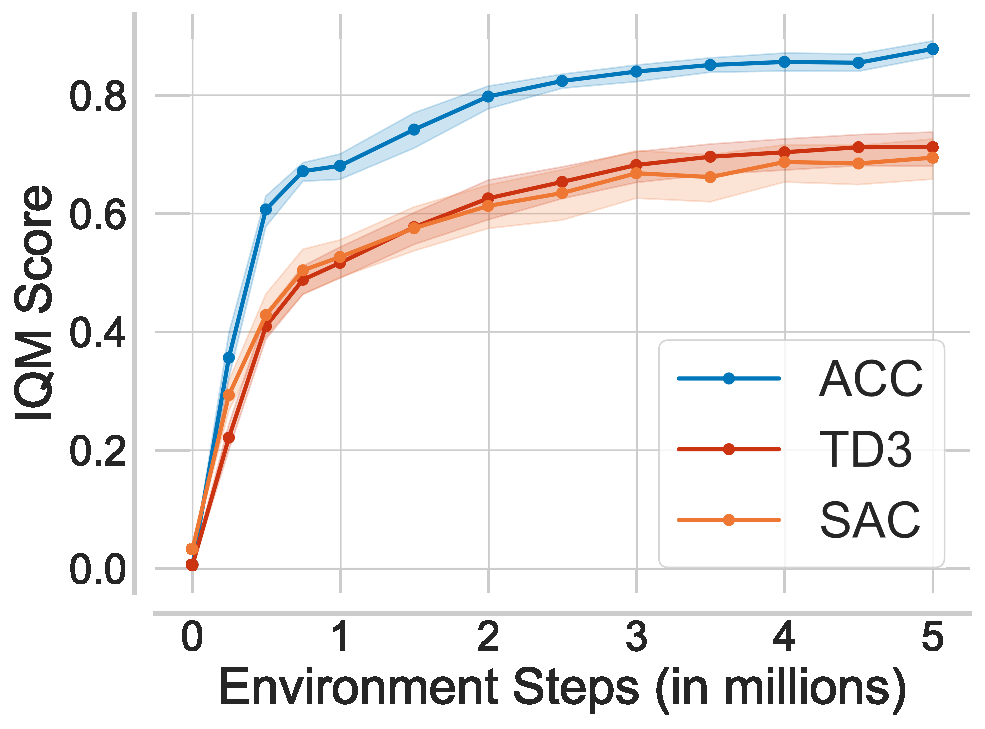
\includegraphics[width=.49\linewidth]{images/main_exp/sac_td3_acc_aggregated_0-eps-converted-to.pdf} &
        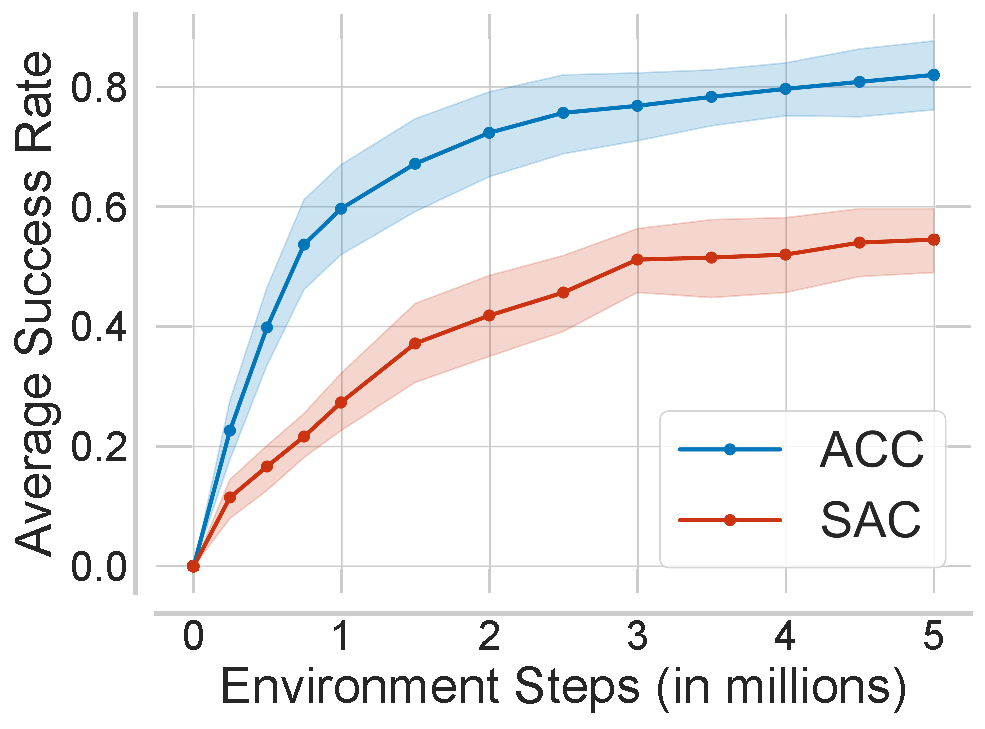
\includegraphics[width= .49\linewidth]{images/main_exp/meta_world_aggregated_mean_std_0-eps-converted-to.pdf} \\
        a) & b) \\
\end{tabular}
\vspace{-0.3cm}
\caption{
Sample efficiency curves aggregated from the results over several environments. The normalized IQM score and the mean of the success rate respectively is plotted against the number of environment steps. Shaded regions denote pointwise $95$\% stratified bootstrap confidence intervals according to the method of \cite{agarwal2021deep}. 
\textbf{(a)} Aggregated results over the $6$ gym continuous control tasks.
\textbf{(b)} Aggregated results over the $12$ metaworld tasks.
}
\label{fig:comparative_aggregated_results}
\vspace{-0.5cm}
\end{figure}


\subsection{Fixing the Number of Dropped Targets}



In this experiment we evaluate how well ACC performs when compared to TQC where the number of dropped targets per network $d$ is fixed to some value.
Since in the original publication for each environment the optimal value was one of the three values $0$, $2$, and $5$, we evaluated TQC with $d$ fixed to one of these values for each environment.
To ensure comparability we used the same codebase as for ACC. 
The results in Figure \ref{fig:ablation_const_number_dropped_atoms_single_curves} show that it is not possible to find one value for $d$ that performs well on all environments.
With $d=0$, TQC is substantially worse on three environments and unstable on the \textit{Ant} environment.
Setting $d=2$ is overall the best choice but still performs clearly worse for two environments and is also slightly worse for \textit{Humanoid}.
Dropping $d=5$ targets per network leads to an algorithm that can compete with ACC only on two of the six environments.
Furthermore, even if there would be one tuned parameter that performs equally well as ACC on a given set of environments we hypothesize there are likely very different environments for which the specific parameter choice will not perform well. The principled nature of ACC on the other hand provides reason to believe that it can perform robustly on a wide range of different environments. This is supported by the robust performance on all considered environments.











\begin{figure}
    \centering
    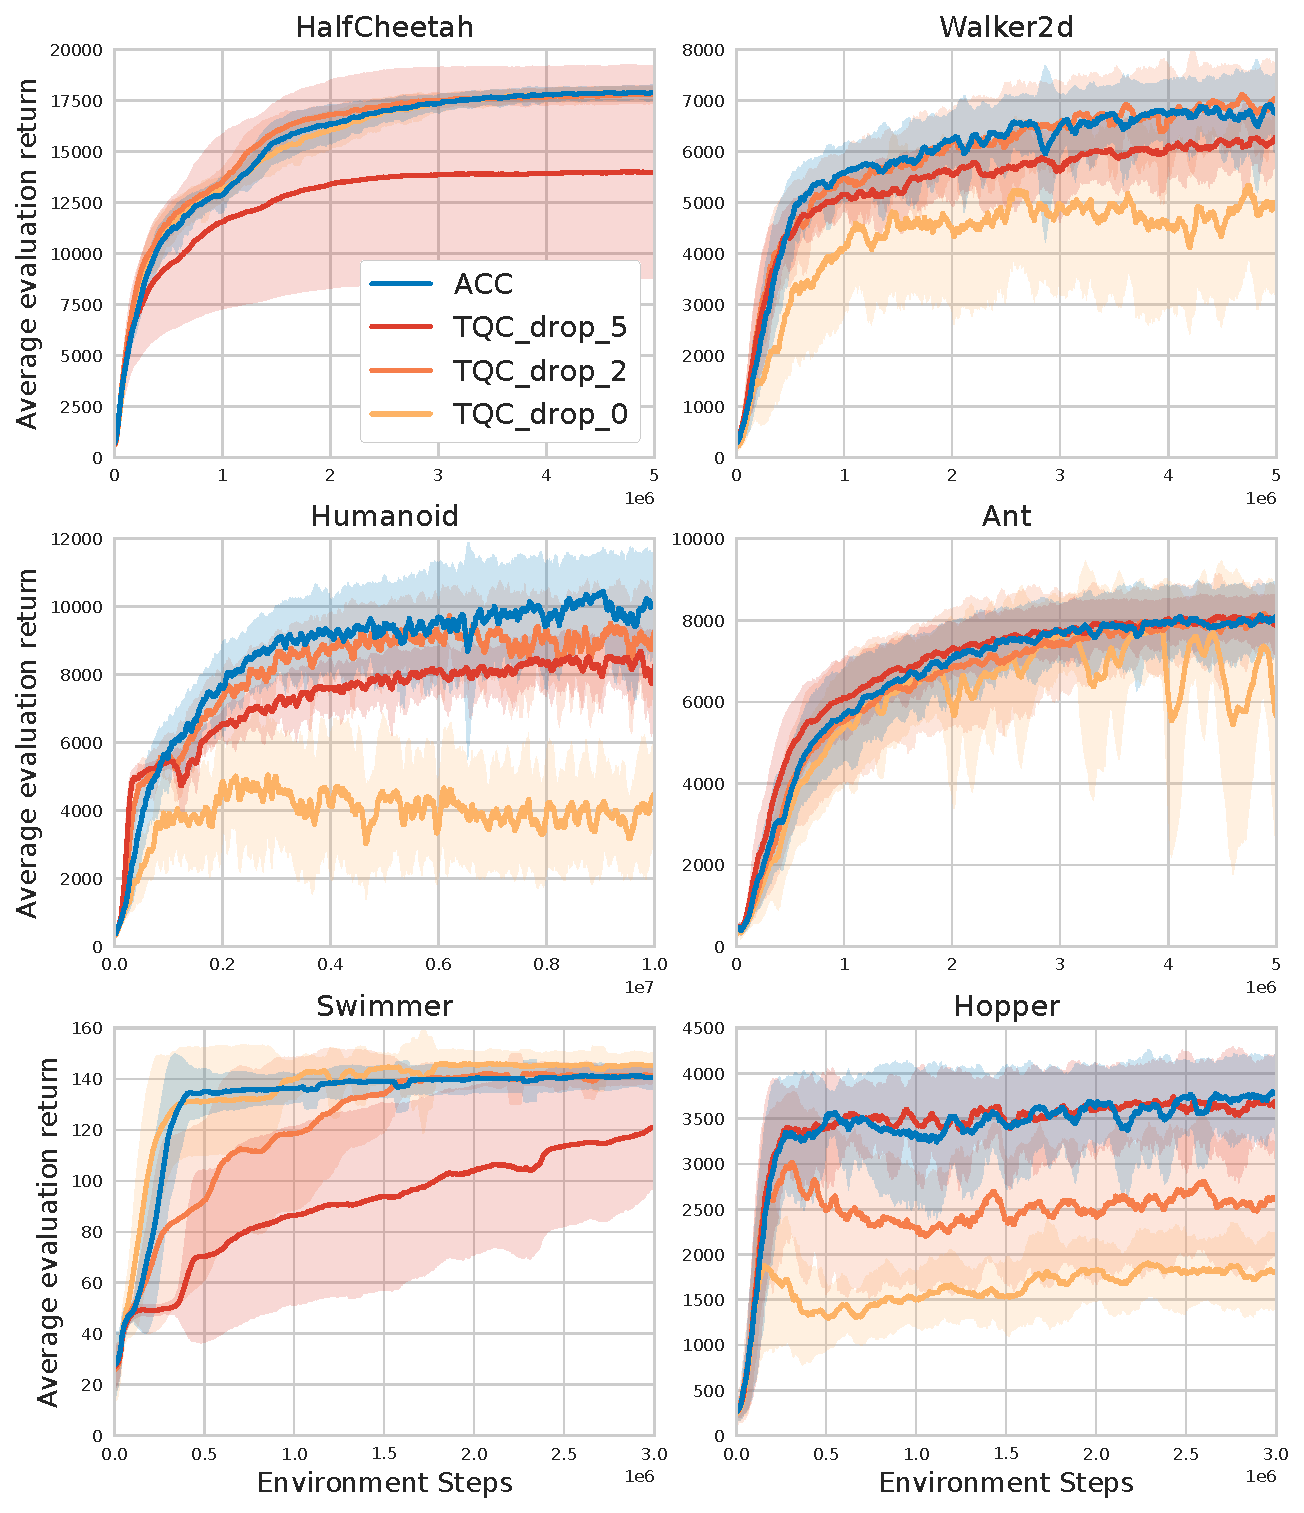
\includegraphics[width=0.93\linewidth]{images/ablation/ablation_const_drop_results_one_fig.pdf}
    \caption{Learning curves of ACC applied to TQC and TQC with different fixed choices for the number of dropped atoms $d$ on six OpenAi gym environments. We used version \textit{v3}. The shaded area represents  mean $\pm$ standard deviation over the $10$ trials. For readability the curves showing the mean are filtered  with a uniform filter of size $15$.}
    \label{fig:ablation_const_number_dropped_atoms_single_curves}
\vspace{-0.5cm}
\end{figure}



\subsection{Evaluation of Sample Efficient Variant}






\begin{figure*}[t]
\footnotesize
\centering 
%\begin{tabular}{P{.56\linewidth}P{.39\linewidth}}
\begin{tabular}{cc}
    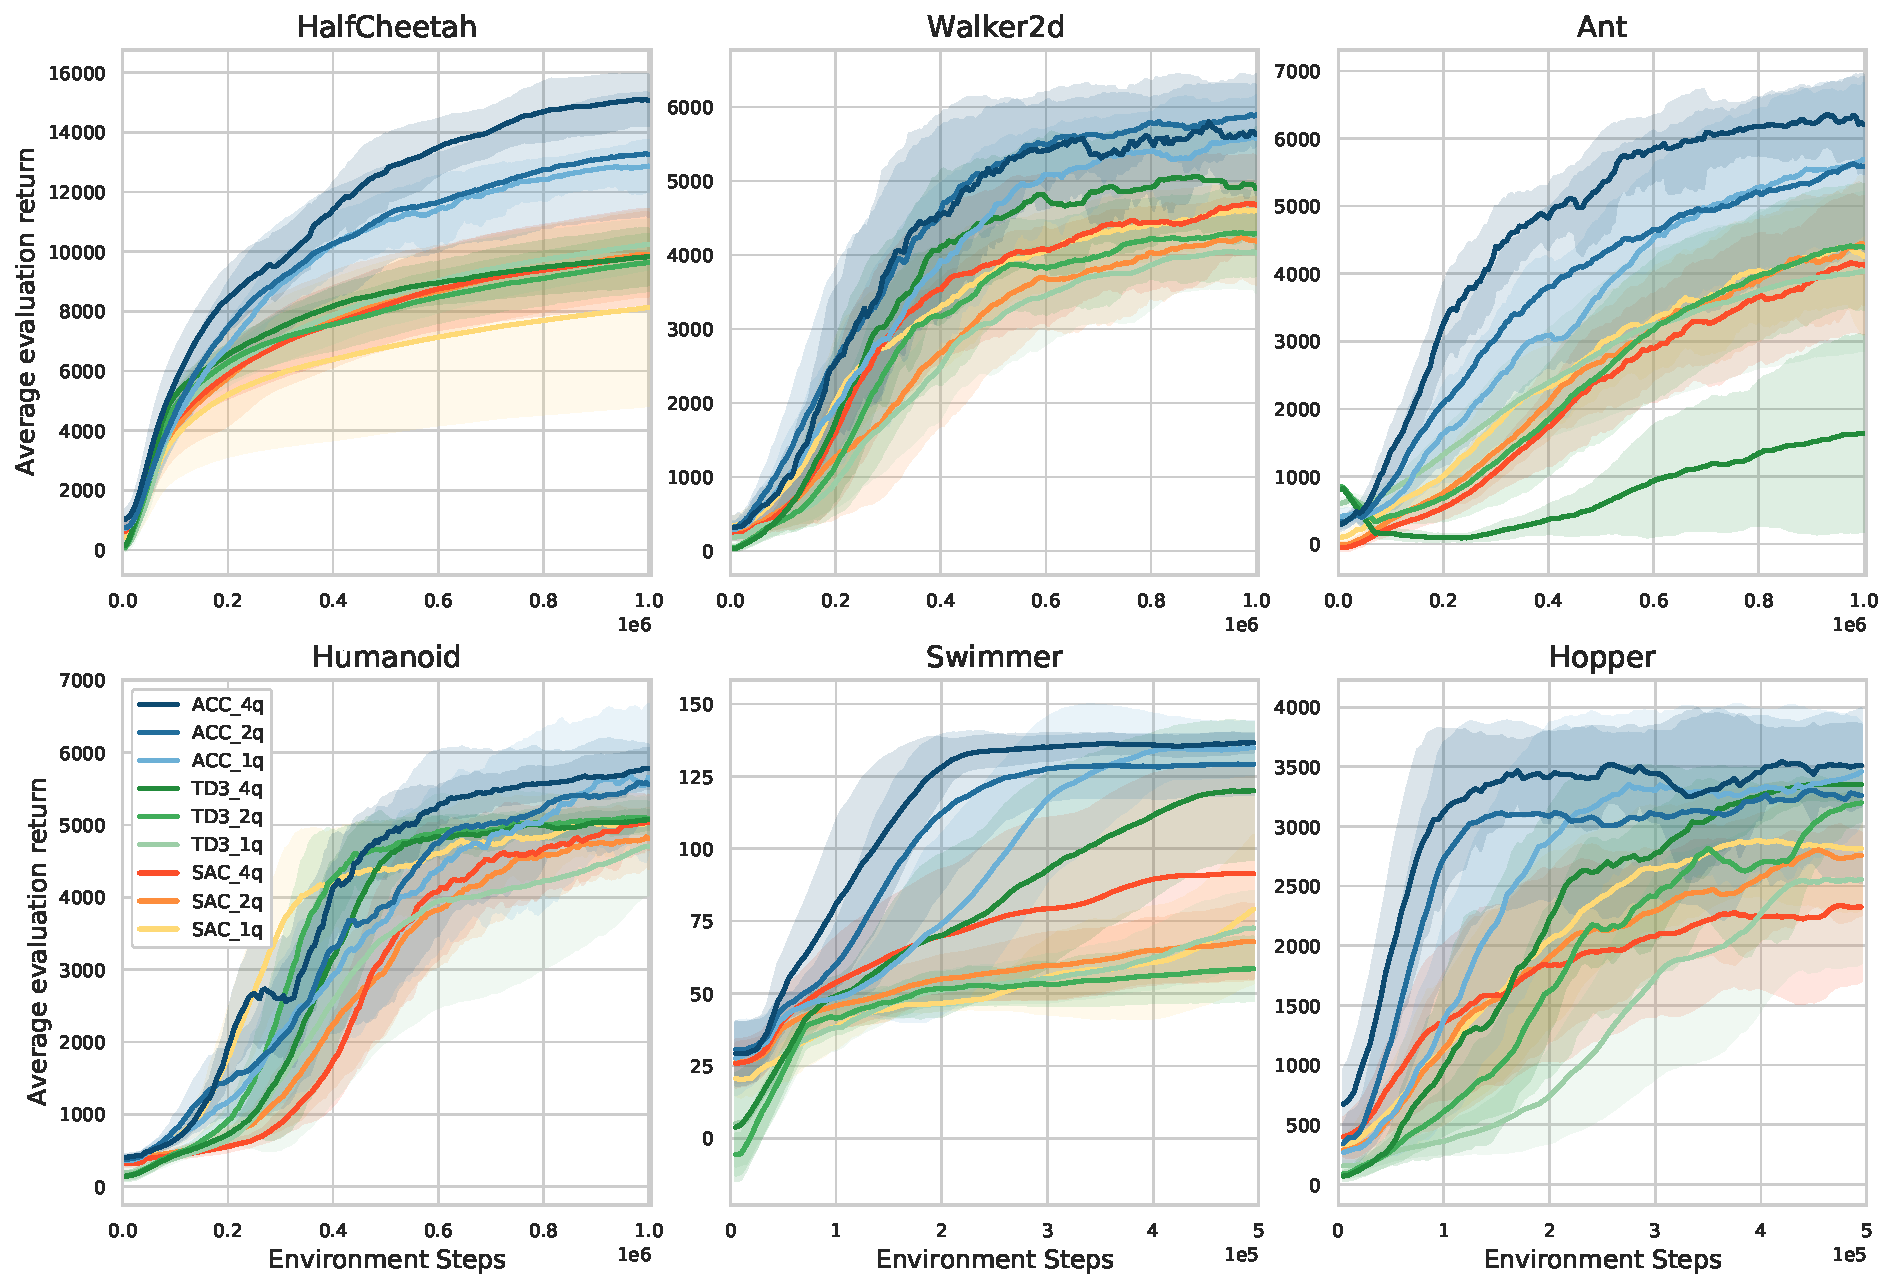
\includegraphics[width=.56\linewidth]{images/less_steps/results_sample_efficient_all_utds_size23.pdf} &
    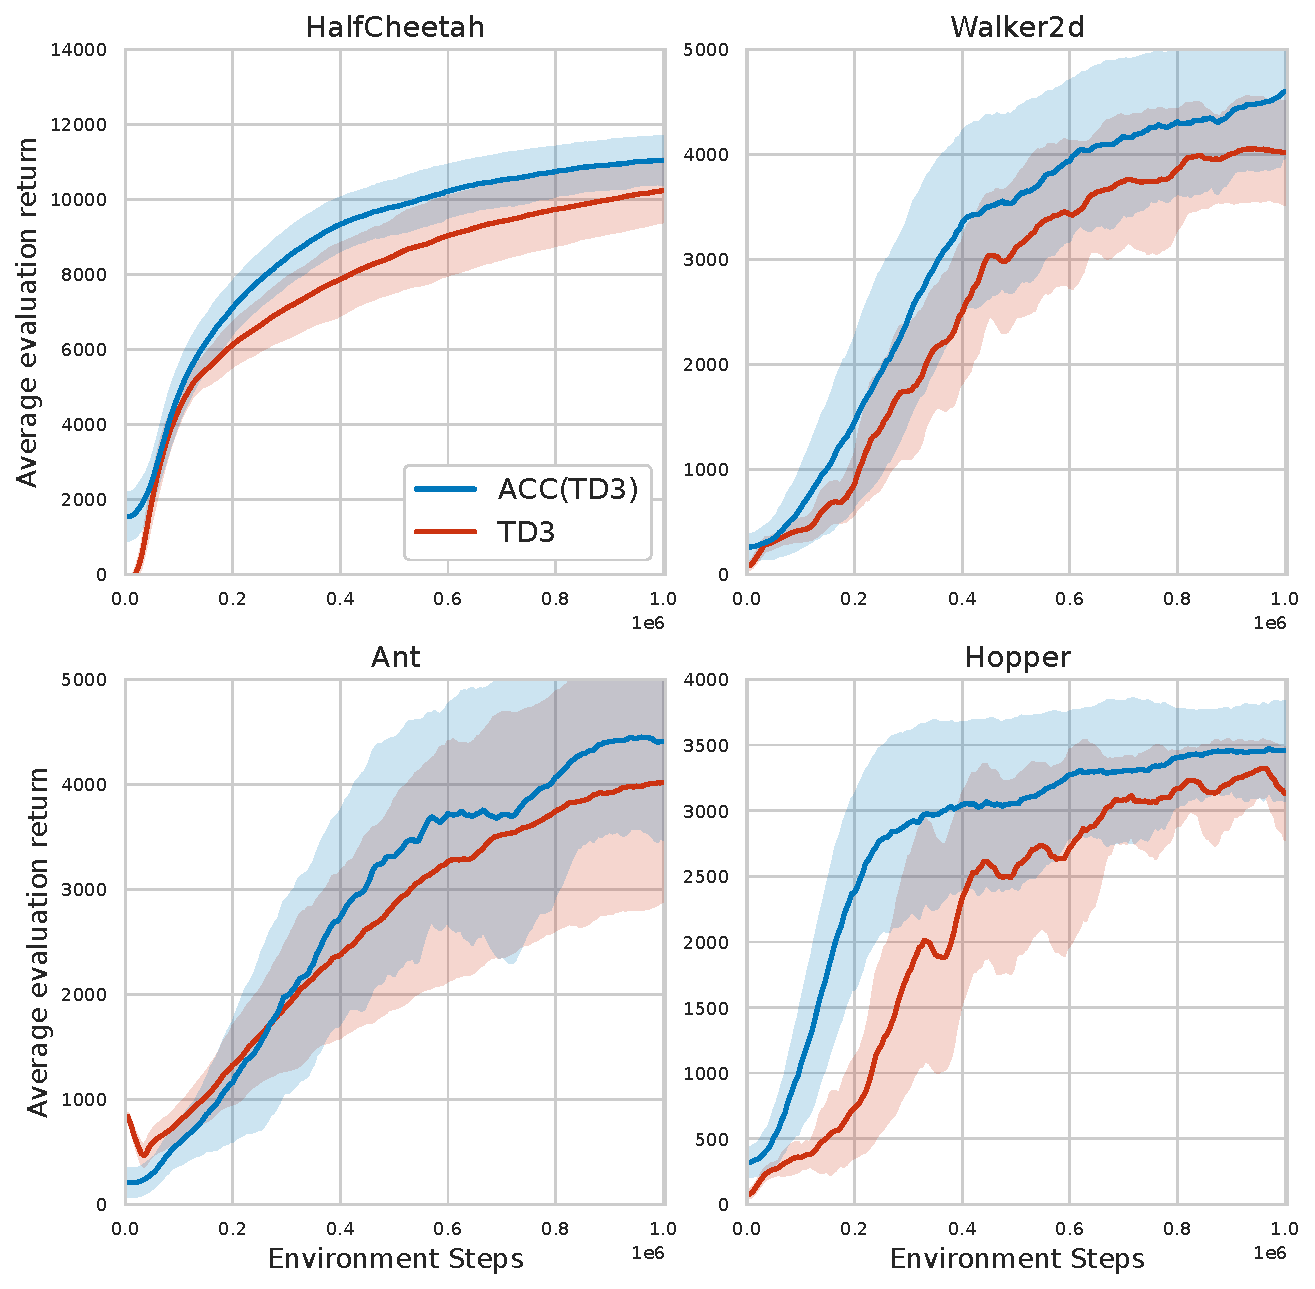
\includegraphics[width=.39\linewidth]{images/main_exp/acc_td3.pdf} \\
    a) & b) \\
\end{tabular}
% \hspace{0mm}
\vspace{-0.3cm}
\caption{
The mean $\pm$ standard deviation over $10$ trials. 
\textbf{(a)} Results in the sample efficient regime where tuning of hyperparameters in an inner loop is too costly with different choices for the number of value function updates per environment step.
\textbf{(b)} Results for ACC applied to TD3 compared to pure TD3.}
\label{fig:further_eval}
\vspace{-0.5cm}
\end{figure*}




In principle more critic updates per environment step should make learning faster. However, because of the bootstrapping in the target computation this can easily become unstable.
The problem is that as targets are changing faster, bias can build up easier and divergence becomes more likely.
ACC provides a way to detect upbuilding bias in the TD targets and to correct the bias accordingly.
This motivates to increase the number of gradient updates of the critic.
In TD3, SAC and TQC one critic update is performed per environment step.
We conducted an experiment to study the effect of increasing this rate up to $4$.
ACC using $4$, $2$ and $1$ updates are denoted with ACC\_4q, ACC\_2q and ACC\_1q respectively. ACC\_1q is equal to ACC from the previous experiments. We use the same notation also for TD3 and SAC.

Scaling the number of critic updates by a factor of $4$ increases the computation time by a factor of $4$. But this can be worthwhile in the sample efficient regime, where a huge number of environment interactions is not possible or the interaction cost dominate the computational costs as it is the case when training robots in the real world.
The results in Figure 
\ref{fig:further_eval}a)
show that in the sample efficient regime ACC4q further increases over plain ACC.
ACC4q reaches the final performance of TD3 and SAC in less than a third of the number of steps for five environments and for \textit{Humanoid} in roughly half the number of steps. 
Increasing the number of critic updates for TD3 and SAC shows mixed results, increasing performance for some environments while decreasing it for others. Only ACC benefits from more updates on all environments, which supports the hypothesis that ACC is successful at calibrating the critic estimate.
% such that the learning dynamics are stable also with more critic updates.

\subsection{Analysis of ACC}


\begin{figure*}[t]
\footnotesize
\centering 
%\begin{tabular}{P{.77\linewidth}P{.22\linewidth}}
\begin{tabular}{cc}
    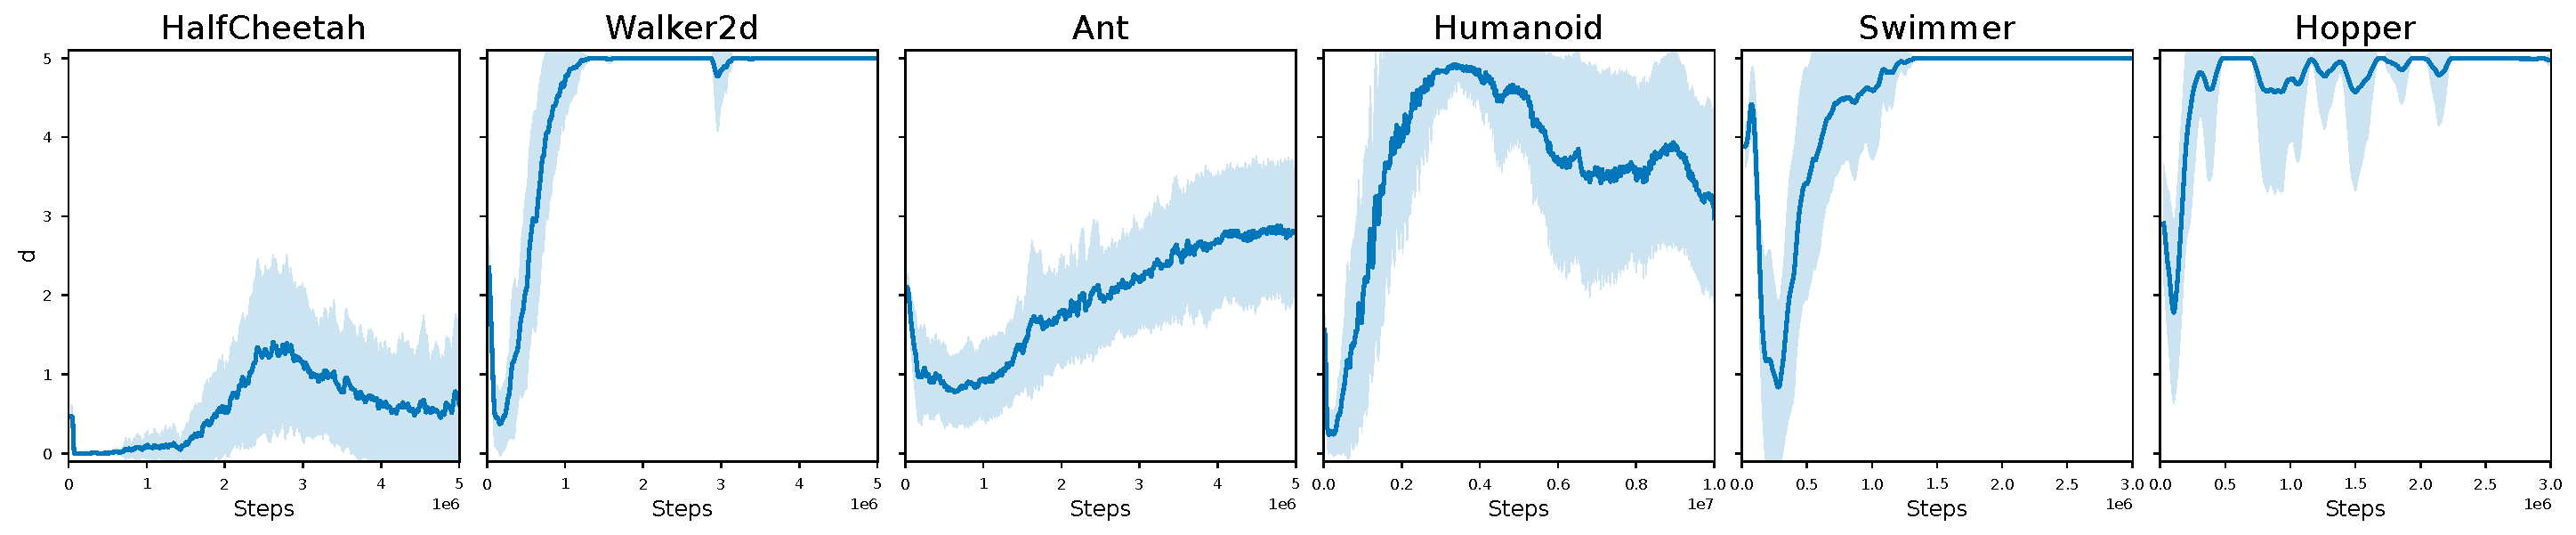
\includegraphics[width=.77\linewidth]{images/analysis/visualize_beta_all_envs.pdf} &
    \hspace{-.4cm}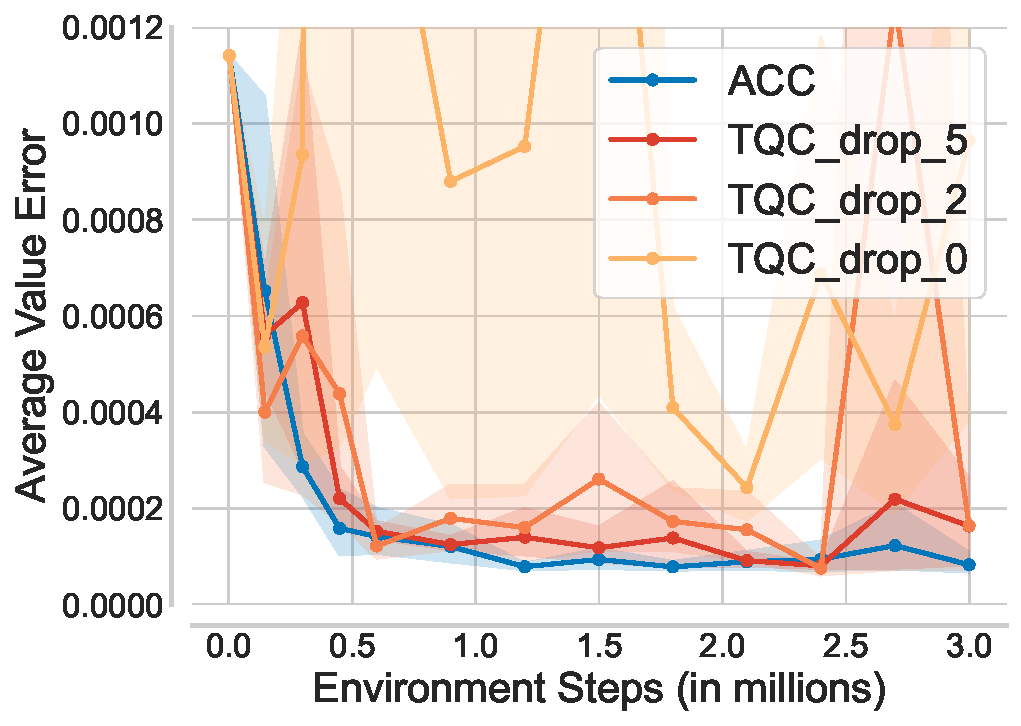
\includegraphics[width=.22\linewidth]{images/analysis/value_error_aggregated_mean_std_0.pdf} \\
    a) & b) \\
\end{tabular}
% \hspace{0mm}
\vspace{-0.3cm}
\caption{
\textbf{(a)} Mean (thick line) and standard deviation (shaded area) over 10 trials of the number of dropped targets per network $d = d_{max} - \beta$ in ACC over time for different environments with a uniform filter of size 15.
\textbf{(b)} The normalized absolute error of the value estimate aggregated over the $6$ environments. Shown are the mean with stratified bootstrapped confidence intervals computed from the results of $5$ trials per environment. We used a uniform filter of size $401$ for readability.}
\label{fig:analysis}
\vspace{-0.5cm}
\end{figure*}

To evaluate the effect of ACC on the bias of the value estimate, we analyze the difference between the value estimate and the corresponding observed return when ACC is applied to TQC.
For each state-action pair encountered during exploration, we compute its value estimate at that time and at the end of the episode compare it  with the actual discounted return from that state onwards. Hence, the state-action pair was not used to update the value function at the point when the value estimate has been computed.
If an episode ends because the maximum number of episode time-steps has been reached, which is 1,000 for the considered environments, we ignore the last $100$ state-action pairs. The reason is that in TQC the value estimator is trained to ignore the episode timeout and uses a bootstrapped target also at the end of the episode. 
We normalize for different value scales by computing the absolute error between the value estimate and the observed discounted return and divide that by the absolute value of the discounted return.
Every 1,000 steps, the average over the errors of the last 1,000 state-action pairs is computed.
The aggregated results in Figure 
\ref{fig:analysis}b)
show that averaged over all environments ACC indeed achieves a lower value error than TQC with the a fixed number of dropped atoms $d$.
This supports our hypothesis that the strong performance of ACC applied to TQC indeed stems from better values estimates.



To better understand the hidden training dynamics of ACC we show in Figure
\ref{fig:analysis}a)
how the number of dropped targets per network $d = d_{max} - \beta$ evolves during training.
Interestingly, the relatively low standard deviation indicates a similar behaviour across runs for a specific environment.
However, there are large differences between the environments which indicates that it might not be possible to find a single hyperparameter that works well on a wide variety of different environments.
Further, the experiments shows that the optimal amount of overestimation correction might change over time during the training even on a single environment.

\subsection{Beyond TQC: Improving TD3 with ACC}

To demonstrate the generality of ACC, we additionally applied it to the actor-critic style TD3 algorithm \cite{td3},
which uses two critics. These are initialized differently but trained with the same target value, which is the minimum over the two targets computed from the two critics.
% This is done to prevent overestimation in the value estimates.
While this successfully prevents the overestimation bias, using the minimum of the two target estimates is very coarse and can instead lead to an underestimation bias.
We applied ACC to TD3 by defining the target for each critic network to be a convex combination between its own target and the minimum over both targets.
Let $Q_i = Q_{\bar{\theta}_i} (s_{t+1}, \pi_{\bar{\phi}} (s_{t+1}) )$, we define the $k$-th critic target
\vspace{-.1cm}
\begin{equation}
\label{eq:td3_target_acc}
    y_k = r + \gamma 
    \Big(   \beta ~ Q_k \nonumber 
     + (1-\beta) \min_{i=1,2} Q_i
    \Big),
\vspace{-.1cm}
\end{equation}
where $\beta \in [0,1]$ is the ACC parameter that is adjusted to balance between under- and overestimation.
The results are displayed in Figure 
\ref{fig:further_eval}b)
and show that ACC also improves the performance of TD3.












